\documentclass[1p]{elsarticle_modified}
%\bibliographystyle{elsarticle-num}

%\usepackage[colorlinks]{hyperref}
%\usepackage{abbrmath_seonhwa} %\Abb, \Ascr, \Acal ,\Abf, \Afrak
\usepackage{amsfonts}
\usepackage{amssymb}
\usepackage{amsmath}
\usepackage{amsthm}
\usepackage{scalefnt}
\usepackage{amsbsy}
\usepackage{kotex}
\usepackage{caption}
\usepackage{subfig}
\usepackage{color}
\usepackage{graphicx}
\usepackage{xcolor} %% white, black, red, green, blue, cyan, magenta, yellow
\usepackage{float}
\usepackage{setspace}
\usepackage{hyperref}

\usepackage{tikz}
\usetikzlibrary{arrows}

\usepackage{multirow}
\usepackage{array} % fixed length table
\usepackage{hhline}

%%%%%%%%%%%%%%%%%%%%%
\makeatletter
\renewcommand*\env@matrix[1][\arraystretch]{%
	\edef\arraystretch{#1}%
	\hskip -\arraycolsep
	\let\@ifnextchar\new@ifnextchar
	\array{*\c@MaxMatrixCols c}}
\makeatother %https://tex.stackexchange.com/questions/14071/how-can-i-increase-the-line-spacing-in-a-matrix
%%%%%%%%%%%%%%%

\usepackage[normalem]{ulem}

\newcommand{\msout}[1]{\ifmmode\text{\sout{\ensuremath{#1}}}\else\sout{#1}\fi}
%SOURCE: \msout is \stkout macro in https://tex.stackexchange.com/questions/20609/strikeout-in-math-mode

\newcommand{\cancel}[1]{
	\ifmmode
	{\color{red}\msout{#1}}
	\else
	{\color{red}\sout{#1}}
	\fi
}

\newcommand{\add}[1]{
	{\color{blue}\uwave{#1}}
}

\newcommand{\replace}[2]{
	\ifmmode
	{\color{red}\msout{#1}}{\color{blue}\uwave{#2}}
	\else
	{\color{red}\sout{#1}}{\color{blue}\uwave{#2}}
	\fi
}

\newcommand{\Sol}{\mathcal{S}} %segment
\newcommand{\D}{D} %diagram
\newcommand{\A}{\mathcal{A}} %arc


%%%%%%%%%%%%%%%%%%%%%%%%%%%%%5 test

\def\sl{\operatorname{\textup{SL}}(2,\Cbb)}
\def\psl{\operatorname{\textup{PSL}}(2,\Cbb)}
\def\quan{\mkern 1mu \triangleright \mkern 1mu}

\theoremstyle{definition}
\newtheorem{thm}{Theorem}[section]
\newtheorem{prop}[thm]{Proposition}
\newtheorem{lem}[thm]{Lemma}
\newtheorem{ques}[thm]{Question}
\newtheorem{cor}[thm]{Corollary}
\newtheorem{defn}[thm]{Definition}
\newtheorem{exam}[thm]{Example}
\newtheorem{rmk}[thm]{Remark}
\newtheorem{alg}[thm]{Algorithm}

\newcommand{\I}{\sqrt{-1}}
\begin{document}

%\begin{frontmatter}
%
%\title{Boundary parabolic representations of knots up to 8 crossings}
%
%%% Group authors per affiliation:
%\author{Yunhi Cho} 
%\address{Department of Mathematics, University of Seoul, Seoul, Korea}
%\ead{yhcho@uos.ac.kr}
%
%
%\author{Seonhwa Kim} %\fnref{s_kim}}
%\address{Center for Geometry and Physics, Institute for Basic Science, Pohang, 37673, Korea}
%\ead{ryeona17@ibs.re.kr}
%
%\author{Hyuk Kim}
%\address{Department of Mathematical Sciences, Seoul National University, Seoul 08826, Korea}
%\ead{hyukkim@snu.ac.kr}
%
%\author{Seokbeom Yoon}
%\address{Department of Mathematical Sciences, Seoul National University, Seoul, 08826,  Korea}
%\ead{sbyoon15@snu.ac.kr}
%
%\begin{abstract}
%We find all boundary parabolic representation of knots up to 8 crossings.
%
%\end{abstract}
%\begin{keyword}
%    \MSC[2010] 57M25 
%\end{keyword}
%
%\end{frontmatter}

%\linenumbers
%\tableofcontents
%
\newcommand\colored[1]{\textcolor{white}{\rule[-0.35ex]{0.8em}{1.4ex}}\kern-0.8em\color{red} #1}%
%\newcommand\colored[1]{\textcolor{white}{ #1}\kern-2.17ex	\textcolor{white}{ #1}\kern-1.81ex	\textcolor{white}{ #1}\kern-2.15ex\color{red}#1	}

{\Large $\underline{12n_{0842}~(K12n_{0842})}$}

\setlength{\tabcolsep}{10pt}
\renewcommand{\arraystretch}{1.6}
\vspace{1cm}\begin{tabular}{m{100pt}>{\centering\arraybackslash}m{274pt}}
\multirow{5}{120pt}{
	\centering
	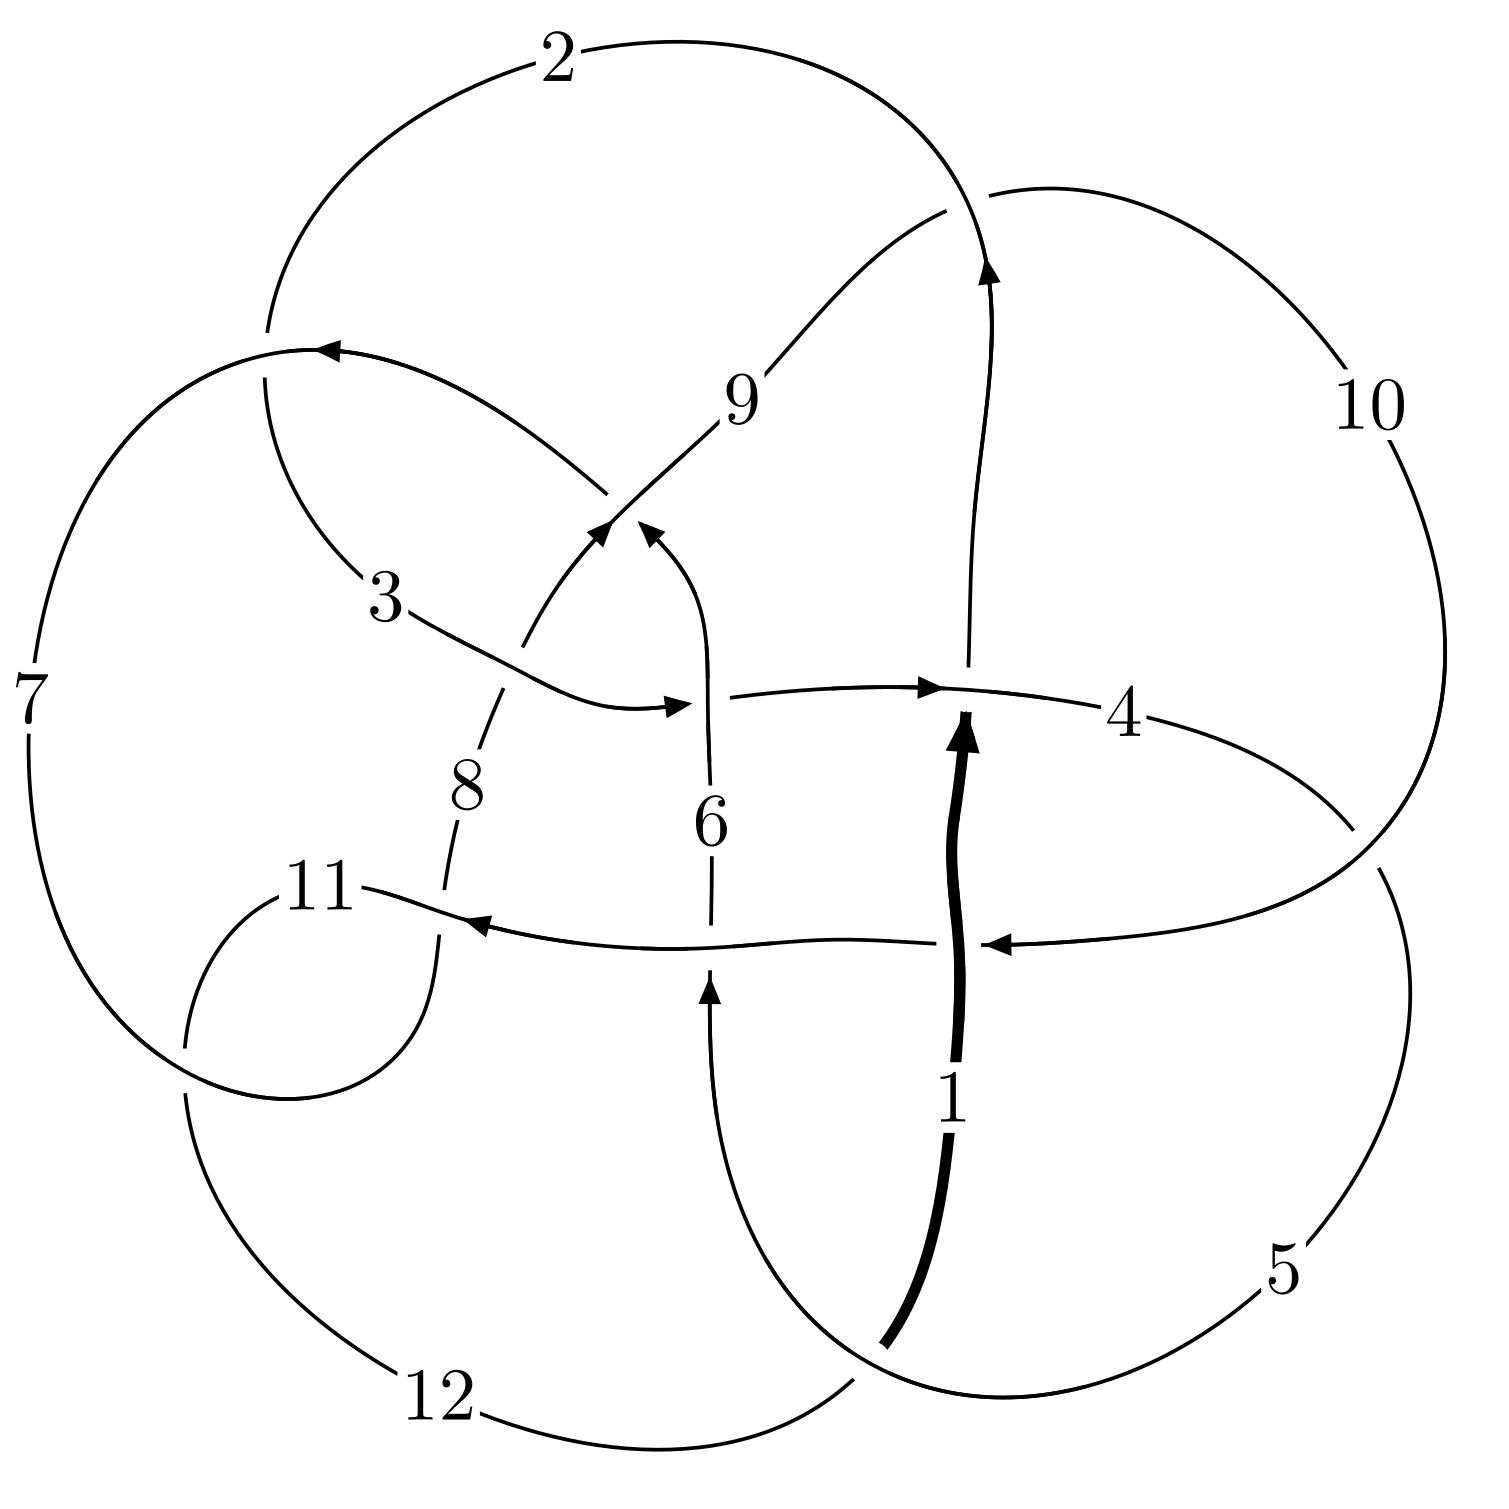
\includegraphics[width=112pt]{../../../GIT/diagram.site/Diagrams/png/2931_12n_0842.png}\\
\ \ \ A knot diagram\footnotemark}&
\allowdisplaybreaks
\textbf{Linearized knot diagam} \\
\cline{2-2}
 &
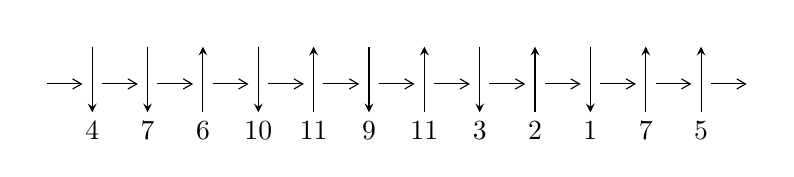
\begin{tikzpicture}[x=20pt, y=17pt]
	% nodes
	\node (C0) at (0, 0) {};
	\node (C1) at (1, 0) {};
	\node (C1U) at (1, +1) {};
	\node (C1D) at (1, -1) {4};

	\node (C2) at (2, 0) {};
	\node (C2U) at (2, +1) {};
	\node (C2D) at (2, -1) {7};

	\node (C3) at (3, 0) {};
	\node (C3U) at (3, +1) {};
	\node (C3D) at (3, -1) {6};

	\node (C4) at (4, 0) {};
	\node (C4U) at (4, +1) {};
	\node (C4D) at (4, -1) {10};

	\node (C5) at (5, 0) {};
	\node (C5U) at (5, +1) {};
	\node (C5D) at (5, -1) {11};

	\node (C6) at (6, 0) {};
	\node (C6U) at (6, +1) {};
	\node (C6D) at (6, -1) {9};

	\node (C7) at (7, 0) {};
	\node (C7U) at (7, +1) {};
	\node (C7D) at (7, -1) {11};

	\node (C8) at (8, 0) {};
	\node (C8U) at (8, +1) {};
	\node (C8D) at (8, -1) {3};

	\node (C9) at (9, 0) {};
	\node (C9U) at (9, +1) {};
	\node (C9D) at (9, -1) {2};

	\node (C10) at (10, 0) {};
	\node (C10U) at (10, +1) {};
	\node (C10D) at (10, -1) {1};

	\node (C11) at (11, 0) {};
	\node (C11U) at (11, +1) {};
	\node (C11D) at (11, -1) {7};

	\node (C12) at (12, 0) {};
	\node (C12U) at (12, +1) {};
	\node (C12D) at (12, -1) {5};
	\node (C13) at (13, 0) {};

	% arrows
	\draw[->,>={angle 60}]
	(C0) edge (C1) (C1) edge (C2) (C2) edge (C3) (C3) edge (C4) (C4) edge (C5) (C5) edge (C6) (C6) edge (C7) (C7) edge (C8) (C8) edge (C9) (C9) edge (C10) (C10) edge (C11) (C11) edge (C12) (C12) edge (C13) ;	\draw[->,>=stealth]
	(C1U) edge (C1D) (C2U) edge (C2D) (C3D) edge (C3U) (C4U) edge (C4D) (C5D) edge (C5U) (C6U) edge (C6D) (C7D) edge (C7U) (C8U) edge (C8D) (C9D) edge (C9U) (C10U) edge (C10D) (C11D) edge (C11U) (C12D) edge (C12U) ;
	\end{tikzpicture} \\
\hhline{~~} \\& 
\textbf{Solving Sequence} \\ \cline{2-2} 
 &
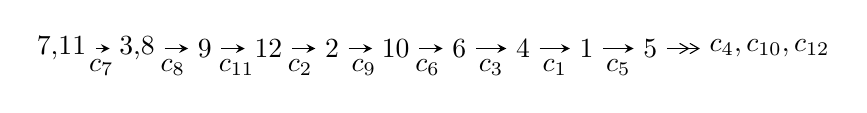
\begin{tikzpicture}[x=23pt, y=7pt]
	% node
	\node (A0) at (-1/8, 0) {7,11};
	\node (A1) at (17/16, 0) {3,8};
	\node (A2) at (17/8, 0) {9};
	\node (A3) at (25/8, 0) {12};
	\node (A4) at (33/8, 0) {2};
	\node (A5) at (41/8, 0) {10};
	\node (A6) at (49/8, 0) {6};
	\node (A7) at (57/8, 0) {4};
	\node (A8) at (65/8, 0) {1};
	\node (A9) at (73/8, 0) {5};
	\node (C1) at (1/2, -1) {$c_{7}$};
	\node (C2) at (13/8, -1) {$c_{8}$};
	\node (C3) at (21/8, -1) {$c_{11}$};
	\node (C4) at (29/8, -1) {$c_{2}$};
	\node (C5) at (37/8, -1) {$c_{9}$};
	\node (C6) at (45/8, -1) {$c_{6}$};
	\node (C7) at (53/8, -1) {$c_{3}$};
	\node (C8) at (61/8, -1) {$c_{1}$};
	\node (C9) at (69/8, -1) {$c_{5}$};
	\node (A10) at (11, 0) {$c_{4},c_{10},c_{12}$};

	% edge
	\draw[->,>=stealth]	
	(A0) edge (A1) (A1) edge (A2) (A2) edge (A3) (A3) edge (A4) (A4) edge (A5) (A5) edge (A6) (A6) edge (A7) (A7) edge (A8) (A8) edge (A9) ;
	\draw[->>,>={angle 60}]	
	(A9) edge (A10);
\end{tikzpicture} \\ 

\end{tabular} \\

\footnotetext{
The image of knot diagram is generated by the software ``\textbf{Draw programme}" developed by Andrew Bartholomew(\url{http://www.layer8.co.uk/maths/draw/index.htm\#Running-draw}), where we modified some parts for our purpose(\url{https://github.com/CATsTAILs/LinksPainter}).
}\phantom \\ \newline 
\centering \textbf{Ideals for irreducible components\footnotemark of $X_{\text{par}}$} 
 
\begin{align*}
I^u_{1}&=\langle 
-1.56702\times10^{964} u^{129}-2.52936\times10^{964} u^{128}+\cdots+1.37131\times10^{968} b-1.84550\times10^{968},\\
\phantom{I^u_{1}}&\phantom{= \langle  }-1.75107\times10^{969} u^{129}-3.48341\times10^{969} u^{128}+\cdots+1.77489\times10^{972} a-2.48142\times10^{973},\\
\phantom{I^u_{1}}&\phantom{= \langle  }u^{130}+2 u^{129}+\cdots+23095 u+1849\rangle \\
I^u_{2}&=\langle 
-2.40523\times10^{66} u^{39}-2.81645\times10^{66} u^{38}+\cdots+8.08698\times10^{65} b+1.18620\times10^{65},\\
\phantom{I^u_{2}}&\phantom{= \langle  }-1.39184\times10^{67} u^{39}+1.04230\times10^{65} u^{38}+\cdots+5.66089\times10^{66} a-7.79024\times10^{67},\;u^{40}+u^{39}+\cdots+2 u-1\rangle \\
\\
\end{align*}
\raggedright * 2 irreducible components of $\dim_{\mathbb{C}}=0$, with total 170 representations.\\
\footnotetext{All coefficients of polynomials are rational numbers. But the coefficients are sometimes approximated in decimal forms when there is not enough margin.}
\newpage
\renewcommand{\arraystretch}{1}
\centering \section*{I. $I^u_{1}= \langle -1.57\times10^{964} u^{129}-2.53\times10^{964} u^{128}+\cdots+1.37\times10^{968} b-1.85\times10^{968},\;-1.75\times10^{969} u^{129}-3.48\times10^{969} u^{128}+\cdots+1.77\times10^{972} a-2.48\times10^{973},\;u^{130}+2 u^{129}+\cdots+23095 u+1849 \rangle$}
\flushleft \textbf{(i) Arc colorings}\\
\begin{tabular}{m{7pt} m{180pt} m{7pt} m{180pt} }
\flushright $a_{7}=$&$\begin{pmatrix}1\\0\end{pmatrix}$ \\
\flushright $a_{11}=$&$\begin{pmatrix}0\\u\end{pmatrix}$ \\
\flushright $a_{3}=$&$\begin{pmatrix}0.000986581 u^{129}+0.00196261 u^{128}+\cdots-75.4998 u+13.9808\\0.000114272 u^{129}+0.000184449 u^{128}+\cdots+12.5203 u+1.34580\end{pmatrix}$ \\
\flushright $a_{8}=$&$\begin{pmatrix}1\\- u^2\end{pmatrix}$ \\
\flushright $a_{9}=$&$\begin{pmatrix}0.00244202 u^{129}+0.00442555 u^{128}+\cdots+289.065 u+25.9338\\0.0000496807 u^{129}+0.000118695 u^{128}+\cdots-8.68282 u-1.28144\end{pmatrix}$ \\
\flushright $a_{12}=$&$\begin{pmatrix}u\\u\end{pmatrix}$ \\
\flushright $a_{2}=$&$\begin{pmatrix}0.00110085 u^{129}+0.00214706 u^{128}+\cdots-62.9795 u+15.3265\\0.000114272 u^{129}+0.000184449 u^{128}+\cdots+12.5203 u+1.34580\end{pmatrix}$ \\
\flushright $a_{10}=$&$\begin{pmatrix}-0.00244447 u^{129}-0.00474242 u^{128}+\cdots-104.893 u-1.82635\\0.000201784 u^{129}+0.000412550 u^{128}+\cdots-8.41360 u+0.410828\end{pmatrix}$ \\
\flushright $a_{6}=$&$\begin{pmatrix}0.00215601 u^{129}+0.00414580 u^{128}+\cdots+132.106 u+13.8909\\-0.000105157 u^{129}-0.000218653 u^{128}+\cdots+6.69702 u-0.156529\end{pmatrix}$ \\
\flushright $a_{4}=$&$\begin{pmatrix}-0.000284206 u^{129}-0.000694296 u^{128}+\cdots-49.4204 u+7.08012\\0.0000830600 u^{129}+0.000168496 u^{128}+\cdots-5.78510 u+0.0521690\end{pmatrix}$ \\
\flushright $a_{1}=$&$\begin{pmatrix}-0.000984849 u^{129}-0.00185266 u^{128}+\cdots+36.5137 u+10.3433\\0.000124562 u^{129}+0.000262122 u^{128}+\cdots-2.40189 u+0.361956\end{pmatrix}$ \\
\flushright $a_{5}=$&$\begin{pmatrix}0.00215601 u^{129}+0.00414580 u^{128}+\cdots+132.106 u+13.8909\\-0.0000495668 u^{129}-0.000106951 u^{128}+\cdots+6.54918 u+0.150793\end{pmatrix}$\\&\end{tabular}
\flushleft \textbf{(ii) Obstruction class $= -1$}\\~\\
\flushleft \textbf{(iii) Cusp Shapes $= 0.0000782799 u^{129}+0.000547387 u^{128}+\cdots-133.386 u-2.54081$}\\~\\
\newpage\renewcommand{\arraystretch}{1}
\flushleft \textbf{(iv) u-Polynomials at the component}\newline \\
\begin{tabular}{m{50pt}|m{274pt}}
Crossings & \hspace{64pt}u-Polynomials at each crossing \\
\hline $$\begin{aligned}c_{1}\end{aligned}$$&$\begin{aligned}
&u^{130}+14 u^{129}+\cdots-159 u+7
\end{aligned}$\\
\hline $$\begin{aligned}c_{2}\end{aligned}$$&$\begin{aligned}
&u^{130}- u^{128}+\cdots-576070405 u+33881141
\end{aligned}$\\
\hline $$\begin{aligned}c_{3}\end{aligned}$$&$\begin{aligned}
&u^{130}-7 u^{129}+\cdots+2725074 u+389673
\end{aligned}$\\
\hline $$\begin{aligned}c_{4}\end{aligned}$$&$\begin{aligned}
&7(7 u^{130}-25 u^{129}+\cdots+12 u+1)
\end{aligned}$\\
\hline $$\begin{aligned}c_{5}\end{aligned}$$&$\begin{aligned}
&7(7 u^{130}+3 u^{129}+\cdots+4.93951\times10^{10} u+2.28860\times10^{9})
\end{aligned}$\\
\hline $$\begin{aligned}c_{6}\end{aligned}$$&$\begin{aligned}
&u^{130}-8 u^{129}+\cdots-205 u+7
\end{aligned}$\\
\hline $$\begin{aligned}c_{7},c_{11}\end{aligned}$$&$\begin{aligned}
&u^{130}+2 u^{129}+\cdots+23095 u+1849
\end{aligned}$\\
\hline $$\begin{aligned}c_{8}\end{aligned}$$&$\begin{aligned}
&7(7 u^{130}-13 u^{129}+\cdots-2351020 u+743993)
\end{aligned}$\\
\hline $$\begin{aligned}c_{9}\end{aligned}$$&$\begin{aligned}
&7(7 u^{130}-34 u^{129}+\cdots-829543 u-30137)
\end{aligned}$\\
\hline $$\begin{aligned}c_{10}\end{aligned}$$&$\begin{aligned}
&u^{130}-9 u^{129}+\cdots-4538 u+203
\end{aligned}$\\
\hline $$\begin{aligned}c_{12}\end{aligned}$$&$\begin{aligned}
&u^{130}+11 u^{129}+\cdots-3169857 u-257957
\end{aligned}$\\
\hline
\end{tabular}\\~\\
\newpage\renewcommand{\arraystretch}{1}
\flushleft \textbf{(v) Riley Polynomials at the component}\newline \\
\begin{tabular}{m{50pt}|m{274pt}}
Crossings & \hspace{64pt}Riley Polynomials at each crossing \\
\hline $$\begin{aligned}c_{1}\end{aligned}$$&$\begin{aligned}
&y^{130}-72 y^{129}+\cdots+493 y+49
\end{aligned}$\\
\hline $$\begin{aligned}c_{2}\end{aligned}$$&$\begin{aligned}
&y^{130}-2 y^{129}+\cdots+55704648955559029 y+1147931715461881
\end{aligned}$\\
\hline $$\begin{aligned}c_{3}\end{aligned}$$&$\begin{aligned}
&y^{130}-39 y^{129}+\cdots-9840220879212 y+151845046929
\end{aligned}$\\
\hline $$\begin{aligned}c_{4}\end{aligned}$$&$\begin{aligned}
&49(49 y^{130}+145 y^{129}+\cdots-314 y+1)
\end{aligned}$\\
\hline $$\begin{aligned}c_{5}\end{aligned}$$&$\begin{aligned}
&49(49 y^{130}-2207 y^{129}+\cdots-2.91410\times10^{20} y+5.23771\times10^{18})
\end{aligned}$\\
\hline $$\begin{aligned}c_{6}\end{aligned}$$&$\begin{aligned}
&y^{130}-28 y^{129}+\cdots-5709 y+49
\end{aligned}$\\
\hline $$\begin{aligned}c_{7},c_{11}\end{aligned}$$&$\begin{aligned}
&y^{130}-96 y^{129}+\cdots+11750551 y+3418801
\end{aligned}$\\
\hline $$\begin{aligned}c_{8}\end{aligned}$$&$\begin{aligned}
&49(49 y^{130}+503 y^{129}+\cdots+5.44033\times10^{13} y+5.53526\times10^{11})
\end{aligned}$\\
\hline $$\begin{aligned}c_{9}\end{aligned}$$&$\begin{aligned}
&49(49 y^{130}+846 y^{129}+\cdots-1.31838\times10^{11} y+9.08239\times10^{8})
\end{aligned}$\\
\hline $$\begin{aligned}c_{10}\end{aligned}$$&$\begin{aligned}
&y^{130}+17 y^{129}+\cdots-739638 y+41209
\end{aligned}$\\
\hline $$\begin{aligned}c_{12}\end{aligned}$$&$\begin{aligned}
&y^{130}-87 y^{129}+\cdots-1836787174947 y+66541813849
\end{aligned}$\\
\hline
\end{tabular}\\~\\
\newpage\flushleft \textbf{(vi) Complex Volumes and Cusp Shapes}
$$\begin{array}{c|c|c}  
\text{Solutions to }I^u_{1}& \I (\text{vol} + \sqrt{-1}CS) & \text{Cusp shape}\\
 \hline 
\begin{aligned}
u &= -0.192985 + 0.987978 I \\
a &= \phantom{-}0.685018 + 0.699135 I \\
b &= \phantom{-}0.105204 + 0.268994 I\end{aligned}
 & -3.85583 + 1.98974 I & \phantom{-0.000000 } 0 \\ \hline\begin{aligned}
u &= -0.192985 - 0.987978 I \\
a &= \phantom{-}0.685018 - 0.699135 I \\
b &= \phantom{-}0.105204 - 0.268994 I\end{aligned}
 & -3.85583 - 1.98974 I & \phantom{-0.000000 } 0 \\ \hline\begin{aligned}
u &= -1.005400 + 0.084588 I \\
a &= -0.424630 - 0.999332 I \\
b &= \phantom{-}1.48759 + 0.21000 I\end{aligned}
 & \phantom{-}3.44265 + 3.95990 I & \phantom{-0.000000 } 0 \\ \hline\begin{aligned}
u &= -1.005400 - 0.084588 I \\
a &= -0.424630 + 0.999332 I \\
b &= \phantom{-}1.48759 - 0.21000 I\end{aligned}
 & \phantom{-}3.44265 - 3.95990 I & \phantom{-0.000000 } 0 \\ \hline\begin{aligned}
u &= \phantom{-}0.982913 + 0.237730 I \\
a &= \phantom{-}0.93751 + 1.73569 I \\
b &= \phantom{-}0.219139 - 0.183732 I\end{aligned}
 & \phantom{-}1.02277 + 1.74041 I & \phantom{-0.000000 } 0 \\ \hline\begin{aligned}
u &= \phantom{-}0.982913 - 0.237730 I \\
a &= \phantom{-}0.93751 - 1.73569 I \\
b &= \phantom{-}0.219139 + 0.183732 I\end{aligned}
 & \phantom{-}1.02277 - 1.74041 I & \phantom{-0.000000 } 0 \\ \hline\begin{aligned}
u &= \phantom{-}1.014750 + 0.047548 I \\
a &= -1.32944 + 0.61104 I \\
b &= -0.746568 - 0.155076 I\end{aligned}
 & \phantom{-}1.73990 - 1.31024 I & \phantom{-0.000000 } 0 \\ \hline\begin{aligned}
u &= \phantom{-}1.014750 - 0.047548 I \\
a &= -1.32944 - 0.61104 I \\
b &= -0.746568 + 0.155076 I\end{aligned}
 & \phantom{-}1.73990 + 1.31024 I & \phantom{-0.000000 } 0 \\ \hline\begin{aligned}
u &= -0.456859 + 0.862239 I \\
a &= -1.287040 - 0.504597 I \\
b &= -0.161070 - 1.105620 I\end{aligned}
 & -2.38775 - 6.44558 I & \phantom{-0.000000 } 0 \\ \hline\begin{aligned}
u &= -0.456859 - 0.862239 I \\
a &= -1.287040 + 0.504597 I \\
b &= -0.161070 + 1.105620 I\end{aligned}
 & -2.38775 + 6.44558 I & \phantom{-0.000000 } 0\\
 \hline 
 \end{array}$$\newpage$$\begin{array}{c|c|c}  
\text{Solutions to }I^u_{1}& \I (\text{vol} + \sqrt{-1}CS) & \text{Cusp shape}\\
 \hline 
\begin{aligned}
u &= -1.054500 + 0.153337 I \\
a &= \phantom{-}0.82634 + 1.70303 I \\
b &= -1.051070 - 0.662151 I\end{aligned}
 & -0.55217 - 6.03667 I & \phantom{-0.000000 } 0 \\ \hline\begin{aligned}
u &= -1.054500 - 0.153337 I \\
a &= \phantom{-}0.82634 - 1.70303 I \\
b &= -1.051070 + 0.662151 I\end{aligned}
 & -0.55217 + 6.03667 I & \phantom{-0.000000 } 0 \\ \hline\begin{aligned}
u &= -1.068270 + 0.127319 I \\
a &= -1.02778 + 1.14025 I \\
b &= \phantom{-}1.26558 - 0.67228 I\end{aligned}
 & \phantom{-}5.94390 - 0.70377 I & \phantom{-0.000000 } 0 \\ \hline\begin{aligned}
u &= -1.068270 - 0.127319 I \\
a &= -1.02778 - 1.14025 I \\
b &= \phantom{-}1.26558 + 0.67228 I\end{aligned}
 & \phantom{-}5.94390 + 0.70377 I & \phantom{-0.000000 } 0 \\ \hline\begin{aligned}
u &= \phantom{-}0.014444 + 1.078290 I \\
a &= \phantom{-}0.087527 + 0.601798 I \\
b &= -0.337332 + 0.607074 I\end{aligned}
 & -3.00735 + 1.68026 I & \phantom{-0.000000 } 0 \\ \hline\begin{aligned}
u &= \phantom{-}0.014444 - 1.078290 I \\
a &= \phantom{-}0.087527 - 0.601798 I \\
b &= -0.337332 - 0.607074 I\end{aligned}
 & -3.00735 - 1.68026 I & \phantom{-0.000000 } 0 \\ \hline\begin{aligned}
u &= -0.709835 + 0.837220 I \\
a &= \phantom{-}0.298449 + 0.444055 I \\
b &= -1.53836 + 1.08055 I\end{aligned}
 & -1.60973 + 3.04444 I & \phantom{-0.000000 } 0 \\ \hline\begin{aligned}
u &= -0.709835 - 0.837220 I \\
a &= \phantom{-}0.298449 - 0.444055 I \\
b &= -1.53836 - 1.08055 I\end{aligned}
 & -1.60973 - 3.04444 I & \phantom{-0.000000 } 0 \\ \hline\begin{aligned}
u &= \phantom{-}0.827680 + 0.118176 I \\
a &= \phantom{-}1.062830 + 0.393846 I \\
b &= \phantom{-}0.578328 - 0.404761 I\end{aligned}
 & \phantom{-}1.72153 + 1.62554 I & \phantom{-0.000000 } 0 \\ \hline\begin{aligned}
u &= \phantom{-}0.827680 - 0.118176 I \\
a &= \phantom{-}1.062830 - 0.393846 I \\
b &= \phantom{-}0.578328 + 0.404761 I\end{aligned}
 & \phantom{-}1.72153 - 1.62554 I & \phantom{-0.000000 } 0\\
 \hline 
 \end{array}$$\newpage$$\begin{array}{c|c|c}  
\text{Solutions to }I^u_{1}& \I (\text{vol} + \sqrt{-1}CS) & \text{Cusp shape}\\
 \hline 
\begin{aligned}
u &= \phantom{-}0.743058 + 0.335777 I \\
a &= \phantom{-}0.985320 + 0.201047 I \\
b &= \phantom{-}0.826366 + 0.263227 I\end{aligned}
 & \phantom{-}1.91444 - 1.66346 I & \phantom{-0.000000 } 0 \\ \hline\begin{aligned}
u &= \phantom{-}0.743058 - 0.335777 I \\
a &= \phantom{-}0.985320 - 0.201047 I \\
b &= \phantom{-}0.826366 - 0.263227 I\end{aligned}
 & \phantom{-}1.91444 + 1.66346 I & \phantom{-0.000000 } 0 \\ \hline\begin{aligned}
u &= -1.215770 + 0.024957 I \\
a &= \phantom{-}0.25672 - 1.77363 I \\
b &= -0.22505 + 2.26759 I\end{aligned}
 & \phantom{-}0.14747 + 3.30778 I & \phantom{-0.000000 } 0 \\ \hline\begin{aligned}
u &= -1.215770 - 0.024957 I \\
a &= \phantom{-}0.25672 + 1.77363 I \\
b &= -0.22505 - 2.26759 I\end{aligned}
 & \phantom{-}0.14747 - 3.30778 I & \phantom{-0.000000 } 0 \\ \hline\begin{aligned}
u &= -1.167050 + 0.344814 I \\
a &= \phantom{-}0.13166 + 1.69916 I \\
b &= -0.91643 - 1.29410 I\end{aligned}
 & \phantom{-}0.35070 - 5.13307 I & \phantom{-0.000000 } 0 \\ \hline\begin{aligned}
u &= -1.167050 - 0.344814 I \\
a &= \phantom{-}0.13166 - 1.69916 I \\
b &= -0.91643 + 1.29410 I\end{aligned}
 & \phantom{-}0.35070 + 5.13307 I & \phantom{-0.000000 } 0 \\ \hline\begin{aligned}
u &= \phantom{-}1.224050 + 0.090932 I \\
a &= \phantom{-}0.605553 - 1.229960 I \\
b &= -0.716654 + 0.669539 I\end{aligned}
 & -1.48112 + 0.30722 I & \phantom{-0.000000 } 0 \\ \hline\begin{aligned}
u &= \phantom{-}1.224050 - 0.090932 I \\
a &= \phantom{-}0.605553 + 1.229960 I \\
b &= -0.716654 - 0.669539 I\end{aligned}
 & -1.48112 - 0.30722 I & \phantom{-0.000000 } 0 \\ \hline\begin{aligned}
u &= \phantom{-}1.157080 + 0.430857 I \\
a &= -0.859745 - 0.586018 I \\
b &= -0.091286 + 0.906175 I\end{aligned}
 & \phantom{-}1.69689 + 1.05048 I & \phantom{-0.000000 } 0 \\ \hline\begin{aligned}
u &= \phantom{-}1.157080 - 0.430857 I \\
a &= -0.859745 + 0.586018 I \\
b &= -0.091286 - 0.906175 I\end{aligned}
 & \phantom{-}1.69689 - 1.05048 I & \phantom{-0.000000 } 0\\
 \hline 
 \end{array}$$\newpage$$\begin{array}{c|c|c}  
\text{Solutions to }I^u_{1}& \I (\text{vol} + \sqrt{-1}CS) & \text{Cusp shape}\\
 \hline 
\begin{aligned}
u &= -0.380261 + 1.187040 I \\
a &= \phantom{-}0.151652 + 0.050180 I \\
b &= -0.080254 - 0.787124 I\end{aligned}
 & \phantom{-}2.16508 + 4.58319 I & \phantom{-0.000000 } 0 \\ \hline\begin{aligned}
u &= -0.380261 - 1.187040 I \\
a &= \phantom{-}0.151652 - 0.050180 I \\
b &= -0.080254 + 0.787124 I\end{aligned}
 & \phantom{-}2.16508 - 4.58319 I & \phantom{-0.000000 } 0 \\ \hline\begin{aligned}
u &= \phantom{-}0.125690 + 1.245530 I \\
a &= \phantom{-}0.075130 + 0.127210 I \\
b &= \phantom{-}0.559438 - 0.639859 I\end{aligned}
 & -0.14578 + 4.97050 I & \phantom{-0.000000 } 0 \\ \hline\begin{aligned}
u &= \phantom{-}0.125690 - 1.245530 I \\
a &= \phantom{-}0.075130 - 0.127210 I \\
b &= \phantom{-}0.559438 + 0.639859 I\end{aligned}
 & -0.14578 - 4.97050 I & \phantom{-0.000000 } 0 \\ \hline\begin{aligned}
u &= \phantom{-}0.116619 + 0.707618 I \\
a &= \phantom{-}0.469121 + 0.190155 I \\
b &= \phantom{-}0.783447 - 0.632126 I\end{aligned}
 & \phantom{-}2.34750 + 2.69810 I & \phantom{-0.000000 } 0 \\ \hline\begin{aligned}
u &= \phantom{-}0.116619 - 0.707618 I \\
a &= \phantom{-}0.469121 - 0.190155 I \\
b &= \phantom{-}0.783447 + 0.632126 I\end{aligned}
 & \phantom{-}2.34750 - 2.69810 I & \phantom{-0.000000 } 0 \\ \hline\begin{aligned}
u &= \phantom{-}1.241780 + 0.360670 I \\
a &= -0.779193 - 0.660654 I \\
b &= \phantom{-}1.015850 + 0.879906 I\end{aligned}
 & \phantom{-}5.19171 + 2.01313 I & \phantom{-0.000000 } 0 \\ \hline\begin{aligned}
u &= \phantom{-}1.241780 - 0.360670 I \\
a &= -0.779193 + 0.660654 I \\
b &= \phantom{-}1.015850 - 0.879906 I\end{aligned}
 & \phantom{-}5.19171 - 2.01313 I & \phantom{-0.000000 } 0 \\ \hline\begin{aligned}
u &= -0.395761 + 1.238470 I \\
a &= -1.67747 + 0.73618 I \\
b &= -1.80089 - 0.24631 I\end{aligned}
 & -4.94996 - 4.30206 I & \phantom{-0.000000 } 0 \\ \hline\begin{aligned}
u &= -0.395761 - 1.238470 I \\
a &= -1.67747 - 0.73618 I \\
b &= -1.80089 + 0.24631 I\end{aligned}
 & -4.94996 + 4.30206 I & \phantom{-0.000000 } 0\\
 \hline 
 \end{array}$$\newpage$$\begin{array}{c|c|c}  
\text{Solutions to }I^u_{1}& \I (\text{vol} + \sqrt{-1}CS) & \text{Cusp shape}\\
 \hline 
\begin{aligned}
u &= \phantom{-}0.343954 + 0.587904 I \\
a &= \phantom{-}0.350168 + 0.631190 I \\
b &= \phantom{-}0.024698 + 0.500867 I\end{aligned}
 & -0.00798 + 1.65365 I & \phantom{-0.000000 } 0 \\ \hline\begin{aligned}
u &= \phantom{-}0.343954 - 0.587904 I \\
a &= \phantom{-}0.350168 - 0.631190 I \\
b &= \phantom{-}0.024698 - 0.500867 I\end{aligned}
 & -0.00798 - 1.65365 I & \phantom{-0.000000 } 0 \\ \hline\begin{aligned}
u &= \phantom{-}0.227794 + 1.302420 I \\
a &= \phantom{-}1.71330 + 0.30061 I \\
b &= \phantom{-}1.306730 - 0.536616 I\end{aligned}
 & -4.09401 + 5.43279 I & \phantom{-0.000000 } 0 \\ \hline\begin{aligned}
u &= \phantom{-}0.227794 - 1.302420 I \\
a &= \phantom{-}1.71330 - 0.30061 I \\
b &= \phantom{-}1.306730 + 0.536616 I\end{aligned}
 & -4.09401 - 5.43279 I & \phantom{-0.000000 } 0 \\ \hline\begin{aligned}
u &= \phantom{-}1.274050 + 0.385225 I \\
a &= \phantom{-}0.763387 + 0.450871 I \\
b &= \phantom{-}0.933879 - 0.338802 I\end{aligned}
 & \phantom{-}1.88232 + 2.39507 I & \phantom{-0.000000 } 0 \\ \hline\begin{aligned}
u &= \phantom{-}1.274050 - 0.385225 I \\
a &= \phantom{-}0.763387 - 0.450871 I \\
b &= \phantom{-}0.933879 + 0.338802 I\end{aligned}
 & \phantom{-}1.88232 - 2.39507 I & \phantom{-0.000000 } 0 \\ \hline\begin{aligned}
u &= -1.328210 + 0.172913 I \\
a &= -0.606992 + 1.142170 I \\
b &= \phantom{-}0.069657 - 0.613093 I\end{aligned}
 & \phantom{-}5.21037 + 2.98126 I & \phantom{-0.000000 } 0 \\ \hline\begin{aligned}
u &= -1.328210 - 0.172913 I \\
a &= -0.606992 - 1.142170 I \\
b &= \phantom{-}0.069657 + 0.613093 I\end{aligned}
 & \phantom{-}5.21037 - 2.98126 I & \phantom{-0.000000 } 0 \\ \hline\begin{aligned}
u &= -1.329800 + 0.240985 I \\
a &= \phantom{-}0.112373 - 1.343230 I \\
b &= \phantom{-}0.279489 + 0.426407 I\end{aligned}
 & \phantom{-}0.56148 - 6.02464 I & \phantom{-0.000000 } 0 \\ \hline\begin{aligned}
u &= -1.329800 - 0.240985 I \\
a &= \phantom{-}0.112373 + 1.343230 I \\
b &= \phantom{-}0.279489 - 0.426407 I\end{aligned}
 & \phantom{-}0.56148 + 6.02464 I & \phantom{-0.000000 } 0\\
 \hline 
 \end{array}$$\newpage$$\begin{array}{c|c|c}  
\text{Solutions to }I^u_{1}& \I (\text{vol} + \sqrt{-1}CS) & \text{Cusp shape}\\
 \hline 
\begin{aligned}
u &= -1.194490 + 0.634915 I \\
a &= \phantom{-}0.38794 - 1.63509 I \\
b &= \phantom{-}1.20321 + 1.03064 I\end{aligned}
 & \phantom{-}5.30423 - 7.34352 I & \phantom{-0.000000 } 0 \\ \hline\begin{aligned}
u &= -1.194490 - 0.634915 I \\
a &= \phantom{-}0.38794 + 1.63509 I \\
b &= \phantom{-}1.20321 - 1.03064 I\end{aligned}
 & \phantom{-}5.30423 + 7.34352 I & \phantom{-0.000000 } 0 \\ \hline\begin{aligned}
u &= \phantom{-}0.402837 + 0.497183 I \\
a &= \phantom{-}0.320224 + 0.850805 I \\
b &= \phantom{-}1.244390 - 0.364572 I\end{aligned}
 & -1.38050 + 5.00016 I & \phantom{-0.000000 } 0. - 9.49193 I \\ \hline\begin{aligned}
u &= \phantom{-}0.402837 - 0.497183 I \\
a &= \phantom{-}0.320224 - 0.850805 I \\
b &= \phantom{-}1.244390 + 0.364572 I\end{aligned}
 & -1.38050 - 5.00016 I & \phantom{-0.000000 -}0. + 9.49193 I \\ \hline\begin{aligned}
u &= \phantom{-}1.372130 + 0.150804 I \\
a &= \phantom{-}0.60945 - 1.47521 I \\
b &= -1.89823 + 1.75461 I\end{aligned}
 & \phantom{-}4.20289 + 8.62109 I & \phantom{-0.000000 } 0 \\ \hline\begin{aligned}
u &= \phantom{-}1.372130 - 0.150804 I \\
a &= \phantom{-}0.60945 + 1.47521 I \\
b &= -1.89823 - 1.75461 I\end{aligned}
 & \phantom{-}4.20289 - 8.62109 I & \phantom{-0.000000 } 0 \\ \hline\begin{aligned}
u &= -1.400810 + 0.159049 I \\
a &= -0.409440 - 1.210060 I \\
b &= \phantom{-}0.606970 + 1.237310 I\end{aligned}
 & -0.26679 - 9.38703 I & \phantom{-0.000000 } 0 \\ \hline\begin{aligned}
u &= -1.400810 - 0.159049 I \\
a &= -0.409440 + 1.210060 I \\
b &= \phantom{-}0.606970 - 1.237310 I\end{aligned}
 & -0.26679 + 9.38703 I & \phantom{-0.000000 } 0 \\ \hline\begin{aligned}
u &= -1.42668\phantom{ +0.000000I} \\
a &= \phantom{-}0.718436\phantom{ +0.000000I} \\
b &= -2.57271\phantom{ +0.000000I}\end{aligned}
 & -0.613003\phantom{ +0.000000I} & \phantom{-0.000000 } 0 \\ \hline\begin{aligned}
u &= -1.30320 + 0.59303 I \\
a &= -0.511695 + 0.877445 I \\
b &= -0.100888 - 0.985304 I\end{aligned}
 & \phantom{-}4.96024 - 4.96838 I & \phantom{-0.000000 } 0\\
 \hline 
 \end{array}$$\newpage$$\begin{array}{c|c|c}  
\text{Solutions to }I^u_{1}& \I (\text{vol} + \sqrt{-1}CS) & \text{Cusp shape}\\
 \hline 
\begin{aligned}
u &= -1.30320 - 0.59303 I \\
a &= -0.511695 - 0.877445 I \\
b &= -0.100888 + 0.985304 I\end{aligned}
 & \phantom{-}4.96024 + 4.96838 I & \phantom{-0.000000 } 0 \\ \hline\begin{aligned}
u &= -0.567677\phantom{ +0.000000I} \\
a &= \phantom{-}0.490107\phantom{ +0.000000I} \\
b &= -1.14200\phantom{ +0.000000I}\end{aligned}
 & -1.77907\phantom{ +0.000000I} & -5.18620\phantom{ +0.000000I} \\ \hline\begin{aligned}
u &= \phantom{-}0.52532 + 1.34589 I \\
a &= \phantom{-}0.473497 + 0.007024 I \\
b &= \phantom{-}0.444301 + 0.616379 I\end{aligned}
 & \phantom{-}0.39548 + 4.33374 I & \phantom{-0.000000 } 0 \\ \hline\begin{aligned}
u &= \phantom{-}0.52532 - 1.34589 I \\
a &= \phantom{-}0.473497 - 0.007024 I \\
b &= \phantom{-}0.444301 - 0.616379 I\end{aligned}
 & \phantom{-}0.39548 - 4.33374 I & \phantom{-0.000000 } 0 \\ \hline\begin{aligned}
u &= -1.41981 + 0.26766 I \\
a &= \phantom{-}0.649756 - 0.389768 I \\
b &= \phantom{-}1.121740 + 0.311792 I\end{aligned}
 & \phantom{-}2.20480 - 10.11460 I & \phantom{-0.000000 } 0 \\ \hline\begin{aligned}
u &= -1.41981 - 0.26766 I \\
a &= \phantom{-}0.649756 + 0.389768 I \\
b &= \phantom{-}1.121740 - 0.311792 I\end{aligned}
 & \phantom{-}2.20480 + 10.11460 I & \phantom{-0.000000 } 0 \\ \hline\begin{aligned}
u &= -1.43085 + 0.21833 I \\
a &= -0.30087 + 1.40417 I \\
b &= \phantom{-}0.08741 - 2.07515 I\end{aligned}
 & \phantom{-}5.80080 - 4.43061 I & \phantom{-0.000000 } 0 \\ \hline\begin{aligned}
u &= -1.43085 - 0.21833 I \\
a &= -0.30087 - 1.40417 I \\
b &= \phantom{-}0.08741 + 2.07515 I\end{aligned}
 & \phantom{-}5.80080 + 4.43061 I & \phantom{-0.000000 } 0 \\ \hline\begin{aligned}
u &= \phantom{-}1.37685 + 0.48002 I \\
a &= -0.221068 - 0.863688 I \\
b &= -0.218612 + 0.767436 I\end{aligned}
 & \phantom{-}4.52979 + 1.33796 I & \phantom{-0.000000 } 0 \\ \hline\begin{aligned}
u &= \phantom{-}1.37685 - 0.48002 I \\
a &= -0.221068 + 0.863688 I \\
b &= -0.218612 - 0.767436 I\end{aligned}
 & \phantom{-}4.52979 - 1.33796 I & \phantom{-0.000000 } 0\\
 \hline 
 \end{array}$$\newpage$$\begin{array}{c|c|c}  
\text{Solutions to }I^u_{1}& \I (\text{vol} + \sqrt{-1}CS) & \text{Cusp shape}\\
 \hline 
\begin{aligned}
u &= -0.349486 + 0.409207 I \\
a &= \phantom{-}1.331860 + 0.024556 I \\
b &= -0.946034 + 0.653814 I\end{aligned}
 & -1.91537 + 1.81462 I & -5.84498 - 1.75098 I \\ \hline\begin{aligned}
u &= -0.349486 - 0.409207 I \\
a &= \phantom{-}1.331860 - 0.024556 I \\
b &= -0.946034 - 0.653814 I\end{aligned}
 & -1.91537 - 1.81462 I & -5.84498 + 1.75098 I \\ \hline\begin{aligned}
u &= -1.40938 + 0.50729 I \\
a &= -0.487450 + 0.765803 I \\
b &= \phantom{-}0.049376 - 0.835322 I\end{aligned}
 & \phantom{-}7.06208 - 1.74086 I & \phantom{-0.000000 } 0 \\ \hline\begin{aligned}
u &= -1.40938 - 0.50729 I \\
a &= -0.487450 - 0.765803 I \\
b &= \phantom{-}0.049376 + 0.835322 I\end{aligned}
 & \phantom{-}7.06208 + 1.74086 I & \phantom{-0.000000 } 0 \\ \hline\begin{aligned}
u &= -1.42183 + 0.48861 I \\
a &= \phantom{-}0.026092 - 1.397180 I \\
b &= \phantom{-}0.95940 + 1.11035 I\end{aligned}
 & \phantom{-}4.87320 - 10.83730 I & \phantom{-0.000000 } 0 \\ \hline\begin{aligned}
u &= -1.42183 - 0.48861 I \\
a &= \phantom{-}0.026092 + 1.397180 I \\
b &= \phantom{-}0.95940 - 1.11035 I\end{aligned}
 & \phantom{-}4.87320 + 10.83730 I & \phantom{-0.000000 } 0 \\ \hline\begin{aligned}
u &= \phantom{-}1.49455 + 0.17001 I \\
a &= \phantom{-}0.941153 + 0.356400 I \\
b &= -2.80546 - 1.08221 I\end{aligned}
 & \phantom{-}2.65451 + 8.61052 I & \phantom{-0.000000 } 0 \\ \hline\begin{aligned}
u &= \phantom{-}1.49455 - 0.17001 I \\
a &= \phantom{-}0.941153 - 0.356400 I \\
b &= -2.80546 + 1.08221 I\end{aligned}
 & \phantom{-}2.65451 - 8.61052 I & \phantom{-0.000000 } 0 \\ \hline\begin{aligned}
u &= -0.28877 + 1.47869 I \\
a &= \phantom{-}0.120770 + 0.123015 I \\
b &= -0.63944 + 1.43069 I\end{aligned}
 & -1.14226 + 3.62625 I & \phantom{-0.000000 } 0 \\ \hline\begin{aligned}
u &= -0.28877 - 1.47869 I \\
a &= \phantom{-}0.120770 - 0.123015 I \\
b &= -0.63944 - 1.43069 I\end{aligned}
 & -1.14226 - 3.62625 I & \phantom{-0.000000 } 0\\
 \hline 
 \end{array}$$\newpage$$\begin{array}{c|c|c}  
\text{Solutions to }I^u_{1}& \I (\text{vol} + \sqrt{-1}CS) & \text{Cusp shape}\\
 \hline 
\begin{aligned}
u &= \phantom{-}1.38195 + 0.60353 I \\
a &= -0.367064 - 0.593723 I \\
b &= \phantom{-}0.016286 + 0.724244 I\end{aligned}
 & \phantom{-}5.55086 + 2.73527 I & \phantom{-0.000000 } 0 \\ \hline\begin{aligned}
u &= \phantom{-}1.38195 - 0.60353 I \\
a &= -0.367064 + 0.593723 I \\
b &= \phantom{-}0.016286 - 0.724244 I\end{aligned}
 & \phantom{-}5.55086 - 2.73527 I & \phantom{-0.000000 } 0 \\ \hline\begin{aligned}
u &= \phantom{-}1.53490\phantom{ +0.000000I} \\
a &= -0.158963\phantom{ +0.000000I} \\
b &= \phantom{-}1.84837\phantom{ +0.000000I}\end{aligned}
 & \phantom{-}1.52550\phantom{ +0.000000I} & \phantom{-0.000000 } 0 \\ \hline\begin{aligned}
u &= \phantom{-}1.55054 + 0.06643 I \\
a &= -0.259009 + 1.059910 I \\
b &= \phantom{-}0.73666 - 1.69771 I\end{aligned}
 & \phantom{-}3.98425 + 2.69852 I & \phantom{-0.000000 } 0 \\ \hline\begin{aligned}
u &= \phantom{-}1.55054 - 0.06643 I \\
a &= -0.259009 - 1.059910 I \\
b &= \phantom{-}0.73666 + 1.69771 I\end{aligned}
 & \phantom{-}3.98425 - 2.69852 I & \phantom{-0.000000 } 0 \\ \hline\begin{aligned}
u &= \phantom{-}0.328062 + 0.289528 I \\
a &= \phantom{-}1.93053 + 0.24387 I \\
b &= \phantom{-}0.236215 + 0.458228 I\end{aligned}
 & \phantom{-}0.65266 + 1.63325 I & \phantom{-}2.68692 - 2.53683 I \\ \hline\begin{aligned}
u &= \phantom{-}0.328062 - 0.289528 I \\
a &= \phantom{-}1.93053 - 0.24387 I \\
b &= \phantom{-}0.236215 - 0.458228 I\end{aligned}
 & \phantom{-}0.65266 - 1.63325 I & \phantom{-}2.68692 + 2.53683 I \\ \hline\begin{aligned}
u &= \phantom{-}1.56708\phantom{ +0.000000I} \\
a &= -0.189228\phantom{ +0.000000I} \\
b &= \phantom{-}1.93649\phantom{ +0.000000I}\end{aligned}
 & \phantom{-}1.52572\phantom{ +0.000000I} & \phantom{-0.000000 } 0 \\ \hline\begin{aligned}
u &= -1.54300 + 0.34814 I \\
a &= \phantom{-}0.068942 + 1.277000 I \\
b &= -0.302820 - 1.262260 I\end{aligned}
 & \phantom{-}7.44054 - 9.96841 I & \phantom{-0.000000 } 0 \\ \hline\begin{aligned}
u &= -1.54300 - 0.34814 I \\
a &= \phantom{-}0.068942 - 1.277000 I \\
b &= -0.302820 + 1.262260 I\end{aligned}
 & \phantom{-}7.44054 + 9.96841 I & \phantom{-0.000000 } 0\\
 \hline 
 \end{array}$$\newpage$$\begin{array}{c|c|c}  
\text{Solutions to }I^u_{1}& \I (\text{vol} + \sqrt{-1}CS) & \text{Cusp shape}\\
 \hline 
\begin{aligned}
u &= \phantom{-}0.364665 + 0.181754 I \\
a &= \phantom{-}0.447705 + 0.540748 I \\
b &= -1.202540 + 0.294643 I\end{aligned}
 & -4.95344 + 0.19459 I & \phantom{-}6.08544 - 3.99455 I \\ \hline\begin{aligned}
u &= \phantom{-}0.364665 - 0.181754 I \\
a &= \phantom{-}0.447705 - 0.540748 I \\
b &= -1.202540 - 0.294643 I\end{aligned}
 & -4.95344 - 0.19459 I & \phantom{-}6.08544 + 3.99455 I \\ \hline\begin{aligned}
u &= -0.357344 + 0.145937 I \\
a &= \phantom{-}0.356206 + 0.571643 I \\
b &= \phantom{-}1.182780 - 0.524412 I\end{aligned}
 & -4.38967 + 8.38798 I & \phantom{-}5.79740 + 1.22412 I \\ \hline\begin{aligned}
u &= -0.357344 - 0.145937 I \\
a &= \phantom{-}0.356206 - 0.571643 I \\
b &= \phantom{-}1.182780 + 0.524412 I\end{aligned}
 & -4.38967 - 8.38798 I & \phantom{-}5.79740 - 1.22412 I \\ \hline\begin{aligned}
u &= \phantom{-}0.08064 + 1.61582 I \\
a &= -0.0950039 - 0.0340072 I \\
b &= -0.274149 - 0.272116 I\end{aligned}
 & -7.81593 + 4.25557 I & \phantom{-0.000000 } 0 \\ \hline\begin{aligned}
u &= \phantom{-}0.08064 - 1.61582 I \\
a &= -0.0950039 + 0.0340072 I \\
b &= -0.274149 + 0.272116 I\end{aligned}
 & -7.81593 - 4.25557 I & \phantom{-0.000000 } 0 \\ \hline\begin{aligned}
u &= \phantom{-}0.26673 + 1.59979 I \\
a &= -0.0224344 - 0.0574521 I \\
b &= -0.72872 - 1.36664 I\end{aligned}
 & \phantom{-}0.00932 - 12.04250 I & \phantom{-0.000000 } 0 \\ \hline\begin{aligned}
u &= \phantom{-}0.26673 - 1.59979 I \\
a &= -0.0224344 + 0.0574521 I \\
b &= -0.72872 + 1.36664 I\end{aligned}
 & \phantom{-}0.00932 + 12.04250 I & \phantom{-0.000000 } 0 \\ \hline\begin{aligned}
u &= -1.42052 + 0.83025 I \\
a &= \phantom{-}0.346397 - 0.701857 I \\
b &= \phantom{-}0.617617 + 0.761177 I\end{aligned}
 & \phantom{-}5.08035 - 12.10800 I & \phantom{-0.000000 } 0 \\ \hline\begin{aligned}
u &= -1.42052 - 0.83025 I \\
a &= \phantom{-}0.346397 + 0.701857 I \\
b &= \phantom{-}0.617617 - 0.761177 I\end{aligned}
 & \phantom{-}5.08035 + 12.10800 I & \phantom{-0.000000 } 0\\
 \hline 
 \end{array}$$\newpage$$\begin{array}{c|c|c}  
\text{Solutions to }I^u_{1}& \I (\text{vol} + \sqrt{-1}CS) & \text{Cusp shape}\\
 \hline 
\begin{aligned}
u &= \phantom{-}1.60096 + 0.41206 I \\
a &= -0.035198 - 1.209550 I \\
b &= -0.55990 + 1.37417 I\end{aligned}
 & \phantom{-}8.41929 + 1.32210 I & \phantom{-0.000000 } 0 \\ \hline\begin{aligned}
u &= \phantom{-}1.60096 - 0.41206 I \\
a &= -0.035198 + 1.209550 I \\
b &= -0.55990 - 1.37417 I\end{aligned}
 & \phantom{-}8.41929 - 1.32210 I & \phantom{-0.000000 } 0 \\ \hline\begin{aligned}
u &= \phantom{-}1.46173 + 0.78033 I \\
a &= \phantom{-}0.365604 + 0.701236 I \\
b &= \phantom{-}0.748972 - 0.841081 I\end{aligned}
 & \phantom{-}3.83692 + 3.90710 I & \phantom{-0.000000 } 0 \\ \hline\begin{aligned}
u &= \phantom{-}1.46173 - 0.78033 I \\
a &= \phantom{-}0.365604 - 0.701236 I \\
b &= \phantom{-}0.748972 + 0.841081 I\end{aligned}
 & \phantom{-}3.83692 - 3.90710 I & \phantom{-0.000000 } 0 \\ \hline\begin{aligned}
u &= -1.67712\phantom{ +0.000000I} \\
a &= -0.248186\phantom{ +0.000000I} \\
b &= -1.61998\phantom{ +0.000000I}\end{aligned}
 & -0.349305\phantom{ +0.000000I} & \phantom{-0.000000 } 0 \\ \hline\begin{aligned}
u &= -0.214366 + 0.220787 I \\
a &= \phantom{-}3.26112 - 2.94875 I \\
b &= \phantom{-}1.163770 + 0.077840 I\end{aligned}
 & -4.09858 + 3.90895 I & -5.63870 - 4.54668 I \\ \hline\begin{aligned}
u &= -0.214366 - 0.220787 I \\
a &= \phantom{-}3.26112 + 2.94875 I \\
b &= \phantom{-}1.163770 - 0.077840 I\end{aligned}
 & -4.09858 - 3.90895 I & -5.63870 + 4.54668 I \\ \hline\begin{aligned}
u &= \phantom{-}0.11947 + 1.69081 I \\
a &= \phantom{-}0.0937528 + 0.0110013 I \\
b &= \phantom{-}0.462723 + 1.325290 I\end{aligned}
 & -0.64061 - 1.41285 I & \phantom{-0.000000 } 0 \\ \hline\begin{aligned}
u &= \phantom{-}0.11947 - 1.69081 I \\
a &= \phantom{-}0.0937528 - 0.0110013 I \\
b &= \phantom{-}0.462723 - 1.325290 I\end{aligned}
 & -0.64061 + 1.41285 I & \phantom{-0.000000 } 0 \\ \hline\begin{aligned}
u &= \phantom{-}1.52387 + 0.75590 I \\
a &= -0.280745 - 1.234770 I \\
b &= -1.26006 + 1.41583 I\end{aligned}
 & \phantom{-}4.1549 + 20.2245 I & \phantom{-0.000000 } 0\\
 \hline 
 \end{array}$$\newpage$$\begin{array}{c|c|c}  
\text{Solutions to }I^u_{1}& \I (\text{vol} + \sqrt{-1}CS) & \text{Cusp shape}\\
 \hline 
\begin{aligned}
u &= \phantom{-}1.52387 - 0.75590 I \\
a &= -0.280745 + 1.234770 I \\
b &= -1.26006 - 1.41583 I\end{aligned}
 & \phantom{-}4.1549 - 20.2245 I & \phantom{-0.000000 } 0 \\ \hline\begin{aligned}
u &= -1.53333 + 0.74990 I \\
a &= -0.283174 + 1.225620 I \\
b &= -1.22937 - 1.56540 I\end{aligned}
 & \phantom{-}2.91524 - 11.64700 I & \phantom{-0.000000 } 0 \\ \hline\begin{aligned}
u &= -1.53333 - 0.74990 I \\
a &= -0.283174 - 1.225620 I \\
b &= -1.22937 + 1.56540 I\end{aligned}
 & \phantom{-}2.91524 + 11.64700 I & \phantom{-0.000000 } 0 \\ \hline\begin{aligned}
u &= -0.260160 + 0.125254 I \\
a &= \phantom{-}2.24562 - 1.13763 I \\
b &= \phantom{-}0.086350 + 0.861525 I\end{aligned}
 & -1.04836 + 3.32741 I & \phantom{-}1.24329 - 3.26995 I \\ \hline\begin{aligned}
u &= -0.260160 - 0.125254 I \\
a &= \phantom{-}2.24562 + 1.13763 I \\
b &= \phantom{-}0.086350 - 0.861525 I\end{aligned}
 & -1.04836 - 3.32741 I & \phantom{-}1.24329 + 3.26995 I \\ \hline\begin{aligned}
u &= \phantom{-}1.51956 + 0.84351 I \\
a &= \phantom{-}0.367911 + 1.152150 I \\
b &= \phantom{-}1.23263 - 1.26490 I\end{aligned}
 & \phantom{-}3.30447 + 10.82410 I & \phantom{-0.000000 } 0 \\ \hline\begin{aligned}
u &= \phantom{-}1.51956 - 0.84351 I \\
a &= \phantom{-}0.367911 - 1.152150 I \\
b &= \phantom{-}1.23263 + 1.26490 I\end{aligned}
 & \phantom{-}3.30447 - 10.82410 I & \phantom{-0.000000 } 0 \\ \hline\begin{aligned}
u &= \phantom{-}1.68007 + 0.45365 I \\
a &= \phantom{-}0.007095 + 1.105530 I \\
b &= \phantom{-}0.95314 - 1.35298 I\end{aligned}
 & \phantom{-}5.51727 + 9.38680 I & \phantom{-0.000000 } 0 \\ \hline\begin{aligned}
u &= \phantom{-}1.68007 - 0.45365 I \\
a &= \phantom{-}0.007095 - 1.105530 I \\
b &= \phantom{-}0.95314 + 1.35298 I\end{aligned}
 & \phantom{-}5.51727 - 9.38680 I & \phantom{-0.000000 } 0 \\ \hline\begin{aligned}
u &= \phantom{-}0.246123 + 0.005560 I \\
a &= \phantom{-}6.60826 + 2.07111 I \\
b &= -1.081240 - 0.595420 I\end{aligned}
 & -0.24013 - 7.66843 I & -2.90470 + 9.94586 I\\
 \hline 
 \end{array}$$\newpage$$\begin{array}{c|c|c}  
\text{Solutions to }I^u_{1}& \I (\text{vol} + \sqrt{-1}CS) & \text{Cusp shape}\\
 \hline 
\begin{aligned}
u &= \phantom{-}0.246123 - 0.005560 I \\
a &= \phantom{-}6.60826 - 2.07111 I \\
b &= -1.081240 + 0.595420 I\end{aligned}
 & -0.24013 + 7.66843 I & -2.90470 - 9.94586 I \\ \hline\begin{aligned}
u &= \phantom{-}1.73414 + 0.44560 I \\
a &= \phantom{-}0.170113 + 0.795594 I \\
b &= \phantom{-}0.57746 - 1.64576 I\end{aligned}
 & \phantom{-}5.26878 + 3.50302 I & \phantom{-0.000000 } 0 \\ \hline\begin{aligned}
u &= \phantom{-}1.73414 - 0.44560 I \\
a &= \phantom{-}0.170113 - 0.795594 I \\
b &= \phantom{-}0.57746 + 1.64576 I\end{aligned}
 & \phantom{-}5.26878 - 3.50302 I & \phantom{-0.000000 } 0 \\ \hline\begin{aligned}
u &= -1.77431 + 0.26416 I \\
a &= \phantom{-}0.201090 - 0.875909 I \\
b &= \phantom{-}0.10396 + 1.61456 I\end{aligned}
 & \phantom{-}7.52045 + 4.51180 I & \phantom{-0.000000 } 0 \\ \hline\begin{aligned}
u &= -1.77431 - 0.26416 I \\
a &= \phantom{-}0.201090 + 0.875909 I \\
b &= \phantom{-}0.10396 - 1.61456 I\end{aligned}
 & \phantom{-}7.52045 - 4.51180 I & \phantom{-0.000000 } 0 \\ \hline\begin{aligned}
u &= -0.146951 + 0.063339 I \\
a &= \phantom{-}16.0501 + 6.7068 I \\
b &= -0.302716 + 0.864166 I\end{aligned}
 & -5.28228 - 0.20426 I & \phantom{-}7.06027 - 2.29073 I \\ \hline\begin{aligned}
u &= -0.146951 - 0.063339 I \\
a &= \phantom{-}16.0501 - 6.7068 I \\
b &= -0.302716 - 0.864166 I\end{aligned}
 & -5.28228 + 0.20426 I & \phantom{-}7.06027 + 2.29073 I \\ \hline\begin{aligned}
u &= -0.0026800 + 0.1179300 I \\
a &= \phantom{-}5.5607 - 28.2192 I \\
b &= -0.080542 - 1.019560 I\end{aligned}
 & -3.42340 + 8.12985 I & \phantom{-}10.41804 + 6.43309 I \\ \hline\begin{aligned}
u &= -0.0026800 - 0.1179300 I \\
a &= \phantom{-}5.5607 + 28.2192 I \\
b &= -0.080542 + 1.019560 I\end{aligned}
 & -3.42340 - 8.12985 I & \phantom{-}10.41804 - 6.43309 I \\ \hline\begin{aligned}
u &= -2.52670\phantom{ +0.000000I} \\
a &= -0.0942858\phantom{ +0.000000I} \\
b &= -2.44028\phantom{ +0.000000I}\end{aligned}
 & -0.402431\phantom{ +0.000000I} & \phantom{-0.000000 } 0\\
 \hline 
 \end{array}$$\newpage\newpage\renewcommand{\arraystretch}{1}
\centering \section*{II. $I^u_{2}= \langle -2.41\times10^{66} u^{39}-2.82\times10^{66} u^{38}+\cdots+8.09\times10^{65} b+1.19\times10^{65},\;-1.39\times10^{67} u^{39}+1.04\times10^{65} u^{38}+\cdots+5.66\times10^{66} a-7.79\times10^{67},\;u^{40}+u^{39}+\cdots+2 u-1 \rangle$}
\flushleft \textbf{(i) Arc colorings}\\
\begin{tabular}{m{7pt} m{180pt} m{7pt} m{180pt} }
\flushright $a_{7}=$&$\begin{pmatrix}1\\0\end{pmatrix}$ \\
\flushright $a_{11}=$&$\begin{pmatrix}0\\u\end{pmatrix}$ \\
\flushright $a_{3}=$&$\begin{pmatrix}2.45870 u^{39}-0.0184122 u^{38}+\cdots-27.5018 u+13.7615\\2.97420 u^{39}+3.48270 u^{38}+\cdots-19.2058 u-0.146681\end{pmatrix}$ \\
\flushright $a_{8}=$&$\begin{pmatrix}1\\- u^2\end{pmatrix}$ \\
\flushright $a_{9}=$&$\begin{pmatrix}-2.55002 u^{39}-2.83592 u^{38}+\cdots+24.0835 u-4.68811\\-0.546160 u^{39}-0.543172 u^{38}+\cdots-3.35179 u+0.405291\end{pmatrix}$ \\
\flushright $a_{12}=$&$\begin{pmatrix}u\\u\end{pmatrix}$ \\
\flushright $a_{2}=$&$\begin{pmatrix}5.43290 u^{39}+3.46429 u^{38}+\cdots-46.7077 u+13.6148\\2.97420 u^{39}+3.48270 u^{38}+\cdots-19.2058 u-0.146681\end{pmatrix}$ \\
\flushright $a_{10}=$&$\begin{pmatrix}-4.63338 u^{39}-2.81760 u^{38}+\cdots+32.0659 u-11.2525\\-2.42174 u^{39}-2.58541 u^{38}+\cdots+1.67460 u-2.14800\end{pmatrix}$ \\
\flushright $a_{6}=$&$\begin{pmatrix}4.57440 u^{39}+5.38104 u^{38}+\cdots-30.5626 u+3.29370\\1.82173 u^{39}+2.41175 u^{38}+\cdots+4.49594 u+0.168550\end{pmatrix}$ \\
\flushright $a_{4}=$&$\begin{pmatrix}-1.60848 u^{39}-4.20407 u^{38}+\cdots+16.8447 u+10.6805\\-5.52043 u^{39}-6.02323 u^{38}+\cdots+42.1526 u-2.77427\end{pmatrix}$ \\
\flushright $a_{1}=$&$\begin{pmatrix}1.81620 u^{39}+1.00198 u^{38}+\cdots-6.47369 u+3.86005\\-2.31703 u^{39}-2.12578 u^{38}+\cdots+31.9391 u-2.36050\end{pmatrix}$ \\
\flushright $a_{5}=$&$\begin{pmatrix}4.57440 u^{39}+5.38104 u^{38}+\cdots-30.5626 u+3.29370\\1.47615 u^{39}+1.83065 u^{38}+\cdots+7.45707 u+0.975187\end{pmatrix}$\\&\end{tabular}
\flushleft \textbf{(ii) Obstruction class $= 1$}\\~\\
\flushleft \textbf{(iii) Cusp Shapes $= 11.0866 u^{39}+19.1437 u^{38}+\cdots-56.3405 u-45.1389$}\\~\\
\newpage\renewcommand{\arraystretch}{1}
\flushleft \textbf{(iv) u-Polynomials at the component}\newline \\
\begin{tabular}{m{50pt}|m{274pt}}
Crossings & \hspace{64pt}u-Polynomials at each crossing \\
\hline $$\begin{aligned}c_{1}\end{aligned}$$&$\begin{aligned}
&u^{40}-23 u^{39}+\cdots+10 u+1
\end{aligned}$\\
\hline $$\begin{aligned}c_{2}\end{aligned}$$&$\begin{aligned}
&u^{40}-3 u^{39}+\cdots-42 u-49
\end{aligned}$\\
\hline $$\begin{aligned}c_{3}\end{aligned}$$&$\begin{aligned}
&u^{40}+8 u^{39}+\cdots+125 u+25
\end{aligned}$\\
\hline $$\begin{aligned}c_{4}\end{aligned}$$&$\begin{aligned}
&7(7 u^{40}+12 u^{39}+\cdots+11 u-1)
\end{aligned}$\\
\hline $$\begin{aligned}c_{5}\end{aligned}$$&$\begin{aligned}
&7(7 u^{40}+12 u^{39}+\cdots+862 u+79)
\end{aligned}$\\
\hline $$\begin{aligned}c_{6}\end{aligned}$$&$\begin{aligned}
&u^{40}-13 u^{39}+\cdots-78 u+7
\end{aligned}$\\
\hline $$\begin{aligned}c_{7}\end{aligned}$$&$\begin{aligned}
&u^{40}+u^{39}+\cdots+2 u-1
\end{aligned}$\\
\hline $$\begin{aligned}c_{8}\end{aligned}$$&$\begin{aligned}
&7(7 u^{40}+10 u^{39}+\cdots+9 u-1)
\end{aligned}$\\
\hline $$\begin{aligned}c_{9}\end{aligned}$$&$\begin{aligned}
&7(7 u^{40}-11 u^{39}+\cdots+26 u-13)
\end{aligned}$\\
\hline $$\begin{aligned}c_{10}\end{aligned}$$&$\begin{aligned}
&u^{40}-10 u^{39}+\cdots+71 u+7
\end{aligned}$\\
\hline $$\begin{aligned}c_{11}\end{aligned}$$&$\begin{aligned}
&u^{40}- u^{39}+\cdots-2 u-1
\end{aligned}$\\
\hline $$\begin{aligned}c_{12}\end{aligned}$$&$\begin{aligned}
&u^{40}-12 u^{39}+\cdots+406 u+49
\end{aligned}$\\
\hline
\end{tabular}\\~\\
\newpage\renewcommand{\arraystretch}{1}
\flushleft \textbf{(v) Riley Polynomials at the component}\newline \\
\begin{tabular}{m{50pt}|m{274pt}}
Crossings & \hspace{64pt}Riley Polynomials at each crossing \\
\hline $$\begin{aligned}c_{1}\end{aligned}$$&$\begin{aligned}
&y^{40}-77 y^{39}+\cdots-40 y+1
\end{aligned}$\\
\hline $$\begin{aligned}c_{2}\end{aligned}$$&$\begin{aligned}
&y^{40}-27 y^{39}+\cdots+41552 y+2401
\end{aligned}$\\
\hline $$\begin{aligned}c_{3}\end{aligned}$$&$\begin{aligned}
&y^{40}-12 y^{39}+\cdots+13975 y+625
\end{aligned}$\\
\hline $$\begin{aligned}c_{4}\end{aligned}$$&$\begin{aligned}
&49(49 y^{40}+220 y^{39}+\cdots-471 y+1)
\end{aligned}$\\
\hline $$\begin{aligned}c_{5}\end{aligned}$$&$\begin{aligned}
&49(49 y^{40}+612 y^{39}+\cdots-443634 y+6241)
\end{aligned}$\\
\hline $$\begin{aligned}c_{6}\end{aligned}$$&$\begin{aligned}
&y^{40}-17 y^{39}+\cdots-302 y+49
\end{aligned}$\\
\hline $$\begin{aligned}c_{7},c_{11}\end{aligned}$$&$\begin{aligned}
&y^{40}-17 y^{39}+\cdots+34 y+1
\end{aligned}$\\
\hline $$\begin{aligned}c_{8}\end{aligned}$$&$\begin{aligned}
&49(49 y^{40}-842 y^{39}+\cdots-43 y+1)
\end{aligned}$\\
\hline $$\begin{aligned}c_{9}\end{aligned}$$&$\begin{aligned}
&49(49 y^{40}+873 y^{39}+\cdots-6526 y+169)
\end{aligned}$\\
\hline $$\begin{aligned}c_{10}\end{aligned}$$&$\begin{aligned}
&y^{40}+4 y^{39}+\cdots-4495 y+49
\end{aligned}$\\
\hline $$\begin{aligned}c_{12}\end{aligned}$$&$\begin{aligned}
&y^{40}-72 y^{39}+\cdots-35280 y+2401
\end{aligned}$\\
\hline
\end{tabular}\\~\\
\newpage\flushleft \textbf{(vi) Complex Volumes and Cusp Shapes}
$$\begin{array}{c|c|c}  
\text{Solutions to }I^u_{2}& \I (\text{vol} + \sqrt{-1}CS) & \text{Cusp shape}\\
 \hline 
\begin{aligned}
u &= \phantom{-}0.985813 + 0.047998 I \\
a &= \phantom{-}1.40863 + 1.55003 I \\
b &= -0.860752 - 0.979037 I\end{aligned}
 & \phantom{-}0.81879 - 7.38277 I & \phantom{-}4.59353 + 7.95478 I \\ \hline\begin{aligned}
u &= \phantom{-}0.985813 - 0.047998 I \\
a &= \phantom{-}1.40863 - 1.55003 I \\
b &= -0.860752 + 0.979037 I\end{aligned}
 & \phantom{-}0.81879 + 7.38277 I & \phantom{-}4.59353 - 7.95478 I \\ \hline\begin{aligned}
u &= -0.140334 + 1.034600 I \\
a &= \phantom{-}0.532953 + 0.635960 I \\
b &= -0.178779 + 0.526366 I\end{aligned}
 & -2.86290 + 2.38388 I & \phantom{-}0.74022 - 10.13995 I \\ \hline\begin{aligned}
u &= -0.140334 - 1.034600 I \\
a &= \phantom{-}0.532953 - 0.635960 I \\
b &= -0.178779 - 0.526366 I\end{aligned}
 & -2.86290 - 2.38388 I & \phantom{-}0.74022 + 10.13995 I \\ \hline\begin{aligned}
u &= \phantom{-}0.270336 + 1.009650 I \\
a &= \phantom{-}2.31571 + 0.91260 I \\
b &= \phantom{-}1.52664 - 0.01344 I\end{aligned}
 & -5.51622 + 4.56551 I & -15.2487 - 6.9844 I \\ \hline\begin{aligned}
u &= \phantom{-}0.270336 - 1.009650 I \\
a &= \phantom{-}2.31571 - 0.91260 I \\
b &= \phantom{-}1.52664 + 0.01344 I\end{aligned}
 & -5.51622 - 4.56551 I & -15.2487 + 6.9844 I \\ \hline\begin{aligned}
u &= -0.900200 + 0.288577 I \\
a &= \phantom{-}1.250680 - 0.514850 I \\
b &= \phantom{-}0.357254 + 0.685349 I\end{aligned}
 & \phantom{-}1.05389 - 1.31798 I & -4.29350 + 4.90343 I \\ \hline\begin{aligned}
u &= -0.900200 - 0.288577 I \\
a &= \phantom{-}1.250680 + 0.514850 I \\
b &= \phantom{-}0.357254 - 0.685349 I\end{aligned}
 & \phantom{-}1.05389 + 1.31798 I & -4.29350 - 4.90343 I \\ \hline\begin{aligned}
u &= -1.103470 + 0.194766 I \\
a &= -0.93591 + 1.46791 I \\
b &= -0.536646 - 0.578625 I\end{aligned}
 & \phantom{-}1.21435 - 2.20942 I & \phantom{-0.000000 -}0. + 8.18325 I \\ \hline\begin{aligned}
u &= -1.103470 - 0.194766 I \\
a &= -0.93591 - 1.46791 I \\
b &= -0.536646 + 0.578625 I\end{aligned}
 & \phantom{-}1.21435 + 2.20942 I & \phantom{-0.000000 } 0. - 8.18325 I\\
 \hline 
 \end{array}$$\newpage$$\begin{array}{c|c|c}  
\text{Solutions to }I^u_{2}& \I (\text{vol} + \sqrt{-1}CS) & \text{Cusp shape}\\
 \hline 
\begin{aligned}
u &= \phantom{-}1.130230 + 0.172412 I \\
a &= -0.903497 - 0.922720 I \\
b &= \phantom{-}1.232620 + 0.608134 I\end{aligned}
 & \phantom{-}5.39290 + 0.98456 I & \phantom{-}1.091376 + 0.161509 I \\ \hline\begin{aligned}
u &= \phantom{-}1.130230 - 0.172412 I \\
a &= -0.903497 + 0.922720 I \\
b &= \phantom{-}1.232620 - 0.608134 I\end{aligned}
 & \phantom{-}5.39290 - 0.98456 I & \phantom{-}1.091376 - 0.161509 I \\ \hline\begin{aligned}
u &= \phantom{-}0.521674 + 1.065710 I \\
a &= -0.168052 + 0.390847 I \\
b &= \phantom{-}1.26221 + 1.24322 I\end{aligned}
 & -1.60771 - 3.26575 I & -10.4994 + 20.1595 I \\ \hline\begin{aligned}
u &= \phantom{-}0.521674 - 1.065710 I \\
a &= -0.168052 - 0.390847 I \\
b &= \phantom{-}1.26221 - 1.24322 I\end{aligned}
 & -1.60771 + 3.26575 I & -10.4994 - 20.1595 I \\ \hline\begin{aligned}
u &= -0.434507 + 1.121790 I \\
a &= -0.430137 - 0.138212 I \\
b &= -0.059769 + 0.349551 I\end{aligned}
 & \phantom{-}0.28364 - 3.88388 I & \phantom{-}1.36521 + 1.74386 I \\ \hline\begin{aligned}
u &= -0.434507 - 1.121790 I \\
a &= -0.430137 + 0.138212 I \\
b &= -0.059769 - 0.349551 I\end{aligned}
 & \phantom{-}0.28364 + 3.88388 I & \phantom{-}1.36521 - 1.74386 I \\ \hline\begin{aligned}
u &= -0.337327 + 1.233090 I \\
a &= -1.69780 + 0.49564 I \\
b &= -1.33154 - 0.74125 I\end{aligned}
 & -4.16063 - 5.13415 I & -6.36747 - 3.09799 I \\ \hline\begin{aligned}
u &= -0.337327 - 1.233090 I \\
a &= -1.69780 - 0.49564 I \\
b &= -1.33154 + 0.74125 I\end{aligned}
 & -4.16063 + 5.13415 I & -6.36747 + 3.09799 I \\ \hline\begin{aligned}
u &= -0.316516 + 0.520550 I \\
a &= -0.46712 + 1.67089 I \\
b &= -1.331820 - 0.186224 I\end{aligned}
 & -2.32747 - 5.29189 I & -6.87764 + 8.97663 I \\ \hline\begin{aligned}
u &= -0.316516 - 0.520550 I \\
a &= -0.46712 - 1.67089 I \\
b &= -1.331820 + 0.186224 I\end{aligned}
 & -2.32747 + 5.29189 I & -6.87764 - 8.97663 I\\
 \hline 
 \end{array}$$\newpage$$\begin{array}{c|c|c}  
\text{Solutions to }I^u_{2}& \I (\text{vol} + \sqrt{-1}CS) & \text{Cusp shape}\\
 \hline 
\begin{aligned}
u &= -1.30916 + 0.55445 I \\
a &= -0.475487 + 0.613831 I \\
b &= \phantom{-}0.215809 - 0.732916 I\end{aligned}
 & \phantom{-}5.30013 - 2.75882 I & \phantom{-0.000000 } 0 \\ \hline\begin{aligned}
u &= -1.30916 - 0.55445 I \\
a &= -0.475487 - 0.613831 I \\
b &= \phantom{-}0.215809 + 0.732916 I\end{aligned}
 & \phantom{-}5.30013 + 2.75882 I & \phantom{-0.000000 } 0 \\ \hline\begin{aligned}
u &= \phantom{-}1.41380 + 0.18507 I \\
a &= \phantom{-}0.590885 - 0.315476 I \\
b &= -2.22284 + 0.16384 I\end{aligned}
 & \phantom{-}3.25291 + 8.75744 I & \phantom{-0.000000 } 0 \\ \hline\begin{aligned}
u &= \phantom{-}1.41380 - 0.18507 I \\
a &= \phantom{-}0.590885 + 0.315476 I \\
b &= -2.22284 - 0.16384 I\end{aligned}
 & \phantom{-}3.25291 - 8.75744 I & \phantom{-0.000000 } 0 \\ \hline\begin{aligned}
u &= -0.075594 + 0.510852 I \\
a &= \phantom{-}0.88648 + 5.00898 I \\
b &= -0.369451 + 0.799053 I\end{aligned}
 & -5.58689 - 0.25968 I & -19.1860 + 2.0754 I \\ \hline\begin{aligned}
u &= -0.075594 - 0.510852 I \\
a &= \phantom{-}0.88648 - 5.00898 I \\
b &= -0.369451 - 0.799053 I\end{aligned}
 & -5.58689 + 0.25968 I & -19.1860 - 2.0754 I \\ \hline\begin{aligned}
u &= \phantom{-}0.179526 + 0.420507 I \\
a &= \phantom{-}4.83757 - 5.63997 I \\
b &= -0.024623 - 1.025940 I\end{aligned}
 & -3.56553 + 8.28671 I & -15.3469 - 21.7718 I \\ \hline\begin{aligned}
u &= \phantom{-}0.179526 - 0.420507 I \\
a &= \phantom{-}4.83757 + 5.63997 I \\
b &= -0.024623 + 1.025940 I\end{aligned}
 & -3.56553 - 8.28671 I & -15.3469 + 21.7718 I \\ \hline\begin{aligned}
u &= -0.06148 + 1.56478 I \\
a &= \phantom{-}0.0566131 - 0.1045900 I \\
b &= \phantom{-}0.338591 - 0.195472 I\end{aligned}
 & -7.89437 - 4.28045 I & \phantom{-0.000000 } 0 \\ \hline\begin{aligned}
u &= -0.06148 - 1.56478 I \\
a &= \phantom{-}0.0566131 + 0.1045900 I \\
b &= \phantom{-}0.338591 + 0.195472 I\end{aligned}
 & -7.89437 + 4.28045 I & \phantom{-0.000000 } 0\\
 \hline 
 \end{array}$$\newpage$$\begin{array}{c|c|c}  
\text{Solutions to }I^u_{2}& \I (\text{vol} + \sqrt{-1}CS) & \text{Cusp shape}\\
 \hline 
\begin{aligned}
u &= \phantom{-}0.006801 + 0.413917 I \\
a &= -0.041680 - 0.840946 I \\
b &= -1.137090 + 0.353354 I\end{aligned}
 & -5.30901 + 0.03558 I & -13.08662 + 3.87514 I \\ \hline\begin{aligned}
u &= \phantom{-}0.006801 - 0.413917 I \\
a &= -0.041680 + 0.840946 I \\
b &= -1.137090 - 0.353354 I\end{aligned}
 & -5.30901 - 0.03558 I & -13.08662 - 3.87514 I \\ \hline\begin{aligned}
u &= \phantom{-}0.160986 + 0.334496 I \\
a &= -0.216404 - 0.977522 I \\
b &= \phantom{-}1.076980 - 0.498814 I\end{aligned}
 & -4.64626 + 8.64955 I & -10.0735 - 14.3657 I \\ \hline\begin{aligned}
u &= \phantom{-}0.160986 - 0.334496 I \\
a &= -0.216404 + 0.977522 I \\
b &= \phantom{-}1.076980 + 0.498814 I\end{aligned}
 & -4.64626 - 8.64955 I & -10.0735 + 14.3657 I \\ \hline\begin{aligned}
u &= \phantom{-}1.52801 + 0.57282 I \\
a &= \phantom{-}0.126503 + 1.248900 I \\
b &= \phantom{-}0.97762 - 1.25745 I\end{aligned}
 & \phantom{-}4.17482 + 9.89074 I & \phantom{-0.000000 } 0 \\ \hline\begin{aligned}
u &= \phantom{-}1.52801 - 0.57282 I \\
a &= \phantom{-}0.126503 - 1.248900 I \\
b &= \phantom{-}0.97762 + 1.25745 I\end{aligned}
 & \phantom{-}4.17482 - 9.89074 I & \phantom{-0.000000 } 0 \\ \hline\begin{aligned}
u &= -1.62923 + 0.38674 I \\
a &= -0.210724 + 0.890348 I \\
b &= -0.40963 - 1.68332 I\end{aligned}
 & \phantom{-}5.07142 - 3.41108 I & \phantom{-0.000000 } 0 \\ \hline\begin{aligned}
u &= -1.62923 - 0.38674 I \\
a &= -0.210724 - 0.890348 I \\
b &= -0.40963 + 1.68332 I\end{aligned}
 & \phantom{-}5.07142 + 3.41108 I & \phantom{-0.000000 } 0 \\ \hline\begin{aligned}
u &= \phantom{-}1.83581\phantom{ +0.000000I} \\
a &= -0.259494\phantom{ +0.000000I} \\
b &= \phantom{-}2.47431\phantom{ +0.000000I}\end{aligned}
 & \phantom{-}1.32808\phantom{ +0.000000I} & \phantom{-0.000000 } 0 \\ \hline\begin{aligned}
u &= -2.61455\phantom{ +0.000000I} \\
a &= -0.0874792\phantom{ +0.000000I} \\
b &= -2.52384\phantom{ +0.000000I}\end{aligned}
 & -0.398487\phantom{ +0.000000I} & \phantom{-0.000000 } 0\\
 \hline 
 \end{array}$$\newpage
\newpage\renewcommand{\arraystretch}{1}
\centering \section*{ III. u-Polynomials}
\begin{tabular}{m{50pt}|m{274pt}}
Crossings & \hspace{64pt}u-Polynomials at each crossing \\
\hline $$\begin{aligned}c_{1}\end{aligned}$$&$\begin{aligned}
&(u^{40}-23 u^{39}+\cdots+10 u+1)(u^{130}+14 u^{129}+\cdots-159 u+7)
\end{aligned}$\\
\hline $$\begin{aligned}c_{2}\end{aligned}$$&$\begin{aligned}
&(u^{40}-3 u^{39}+\cdots-42 u-49)\\
&\cdot(u^{130}- u^{128}+\cdots-576070405 u+33881141)
\end{aligned}$\\
\hline $$\begin{aligned}c_{3}\end{aligned}$$&$\begin{aligned}
&(u^{40}+8 u^{39}+\cdots+125 u+25)\\
&\cdot(u^{130}-7 u^{129}+\cdots+2725074 u+389673)
\end{aligned}$\\
\hline $$\begin{aligned}c_{4}\end{aligned}$$&$\begin{aligned}
&49(7 u^{40}+12 u^{39}+\cdots+11 u-1)(7 u^{130}-25 u^{129}+\cdots+12 u+1)
\end{aligned}$\\
\hline $$\begin{aligned}c_{5}\end{aligned}$$&$\begin{aligned}
&49(7 u^{40}+12 u^{39}+\cdots+862 u+79)\\
&\cdot(7 u^{130}+3 u^{129}+\cdots+49395145991 u+2288603579)
\end{aligned}$\\
\hline $$\begin{aligned}c_{6}\end{aligned}$$&$\begin{aligned}
&(u^{40}-13 u^{39}+\cdots-78 u+7)(u^{130}-8 u^{129}+\cdots-205 u+7)
\end{aligned}$\\
\hline $$\begin{aligned}c_{7}\end{aligned}$$&$\begin{aligned}
&(u^{40}+u^{39}+\cdots+2 u-1)(u^{130}+2 u^{129}+\cdots+23095 u+1849)
\end{aligned}$\\
\hline $$\begin{aligned}c_{8}\end{aligned}$$&$\begin{aligned}
&49(7 u^{40}+10 u^{39}+\cdots+9 u-1)\\
&\cdot(7 u^{130}-13 u^{129}+\cdots-2351020 u+743993)
\end{aligned}$\\
\hline $$\begin{aligned}c_{9}\end{aligned}$$&$\begin{aligned}
&49(7 u^{40}-11 u^{39}+\cdots+26 u-13)\\
&\cdot(7 u^{130}-34 u^{129}+\cdots-829543 u-30137)
\end{aligned}$\\
\hline $$\begin{aligned}c_{10}\end{aligned}$$&$\begin{aligned}
&(u^{40}-10 u^{39}+\cdots+71 u+7)(u^{130}-9 u^{129}+\cdots-4538 u+203)
\end{aligned}$\\
\hline $$\begin{aligned}c_{11}\end{aligned}$$&$\begin{aligned}
&(u^{40}- u^{39}+\cdots-2 u-1)(u^{130}+2 u^{129}+\cdots+23095 u+1849)
\end{aligned}$\\
\hline $$\begin{aligned}c_{12}\end{aligned}$$&$\begin{aligned}
&(u^{40}-12 u^{39}+\cdots+406 u+49)\\
&\cdot(u^{130}+11 u^{129}+\cdots-3169857 u-257957)
\end{aligned}$\\
\hline
\end{tabular}\newpage\renewcommand{\arraystretch}{1}
\centering \section*{ IV. Riley Polynomials}
\begin{tabular}{m{50pt}|m{274pt}}
Crossings & \hspace{64pt}Riley Polynomials at each crossing \\
\hline $$\begin{aligned}c_{1}\end{aligned}$$&$\begin{aligned}
&(y^{40}-77 y^{39}+\cdots-40 y+1)(y^{130}-72 y^{129}+\cdots+493 y+49)
\end{aligned}$\\
\hline $$\begin{aligned}c_{2}\end{aligned}$$&$\begin{aligned}
&(y^{40}-27 y^{39}+\cdots+41552 y+2401)\\
&\cdot(y^{130}-2 y^{129}+\cdots+55704648955559029 y+1147931715461881)
\end{aligned}$\\
\hline $$\begin{aligned}c_{3}\end{aligned}$$&$\begin{aligned}
&(y^{40}-12 y^{39}+\cdots+13975 y+625)\\
&\cdot(y^{130}-39 y^{129}+\cdots-9840220879212 y+151845046929)
\end{aligned}$\\
\hline $$\begin{aligned}c_{4}\end{aligned}$$&$\begin{aligned}
&2401(49 y^{40}+220 y^{39}+\cdots-471 y+1)\\
&\cdot(49 y^{130}+145 y^{129}+\cdots-314 y+1)
\end{aligned}$\\
\hline $$\begin{aligned}c_{5}\end{aligned}$$&$\begin{aligned}
&2401(49 y^{40}+612 y^{39}+\cdots-443634 y+6241)\\
&\cdot(49 y^{130}-2207 y^{129}+\cdots-2.91\times10^{20} y+5.24\times10^{18})
\end{aligned}$\\
\hline $$\begin{aligned}c_{6}\end{aligned}$$&$\begin{aligned}
&(y^{40}-17 y^{39}+\cdots-302 y+49)(y^{130}-28 y^{129}+\cdots-5709 y+49)
\end{aligned}$\\
\hline $$\begin{aligned}c_{7},c_{11}\end{aligned}$$&$\begin{aligned}
&(y^{40}-17 y^{39}+\cdots+34 y+1)\\
&\cdot(y^{130}-96 y^{129}+\cdots+11750551 y+3418801)
\end{aligned}$\\
\hline $$\begin{aligned}c_{8}\end{aligned}$$&$\begin{aligned}
&2401(49 y^{40}-842 y^{39}+\cdots-43 y+1)\\
&\cdot(49 y^{130}+503 y^{129}+\cdots+54403265075498 y+553525584049)
\end{aligned}$\\
\hline $$\begin{aligned}c_{9}\end{aligned}$$&$\begin{aligned}
&2401(49 y^{40}+873 y^{39}+\cdots-6526 y+169)\\
&\cdot(49 y^{130}+846 y^{129}+\cdots-131837763381 y+908238769)
\end{aligned}$\\
\hline $$\begin{aligned}c_{10}\end{aligned}$$&$\begin{aligned}
&(y^{40}+4 y^{39}+\cdots-4495 y+49)\\
&\cdot(y^{130}+17 y^{129}+\cdots-739638 y+41209)
\end{aligned}$\\
\hline $$\begin{aligned}c_{12}\end{aligned}$$&$\begin{aligned}
&(y^{40}-72 y^{39}+\cdots-35280 y+2401)\\
&\cdot(y^{130}-87 y^{129}+\cdots-1836787174947 y+66541813849)
\end{aligned}$\\
\hline
\end{tabular}
\vskip 2pc
\end{document}